\documentclass[11pt]{article}
%%%%%%%%%%%%%%%%%%%%%%%%%%%%%%%%%%%%%%%%%

\usepackage{amscd}
\usepackage{amsmath}
\usepackage{amssymb}
\usepackage{amsthm}


\usepackage{epsfig}
\usepackage{verbatim}
\usepackage{graphicx}
\usepackage{amsthm}
\usepackage{hyperref}
\pagestyle{empty}
\usepackage{color}
\usepackage[left=0.75in,top=0.35in,right=0.75in,bottom=0.35in]{geometry} % Document margins
%\usepackage[all,dvips]{xy}


\begin{comment}  

This LaTeX document is a template to be used by Bates mathematics rising seniors to create a thesis proposal. 

As a guide, the document is already filled out to represent a fictitious proposal, and all you need to do is modify the entries below to represent your own proposal.

A PDF version of the fictitious proposal is available on the department's FAQ and Policies pages, at
http://abacus.bates.edu/acad/depts/math/faq.html
and
http://abacus.bates.edu/acad/depts/math/policies.html
respectively.

Once you have finished your proposal, export it to a PDF file. Give the file a USEFUL name, for example, RiemannThesisProposal.PDF. Email the PDF file to Clementine Brasier, the 
Academic Administrative Assistant for Hathorn Hall, at cbrasier\@bates.edu

This LaTex document was created Feb/Mar 2010 by Adriana Salerno and updated Feb 2012 by Meredith Greer

\end{comment}


%\setlength{\textheight}{8.5in} \setlength{\topmargin}{0.0in}
%\setlength{\headheight}{0.0in} \setlength{\headsep}{0.0in}
%\setlength{\leftmargin}{0.0in}
%\setlength{\oddsidemargin}{0.0in}
%%\setlength{\parindent}{1pc}
%\setlength{\textwidth}{6.5in}
%%\linespread{1.6}

\newtheorem{definition}{Definition}
\newtheorem{problem}{Problem}

\newtheorem{theorem}{Theorem}[section]
\newtheorem{lemma}[theorem]{Lemma}
\newtheorem{note}[theorem]{Note}
\newtheorem{corollary}[theorem]{Corollary}
\newtheorem{prop}[theorem]{Proposition}

%%%%%%%%%%%%%%%%%%%%%%%%%%%%%%%%%%%%%%%%%

\begin{document}
	\thispagestyle{empty}
	
	
	\centerline{\textbf{\Large{Mining Yelp reviews}}}
	
	\bigskip
	
	\noindent \textbf{Authors:} 
	Aditya Priyadarshi, Abhay Kasturia, Xingxing Liu, Varun Nandu and Gautam Vashisht
	
	\bigskip
	
	\noindent \textbf{Problem Description:} 
	The objective of this project to analyze yelp reviews dataset \cite{yelp} and build a recommendation system to suggest businesses to users based on their earlier reviews.
	
	\bigskip 
	
	\noindent \textbf{Summary of Data:} 
	The original dataset described in the Yelp Dataset Challenge 10 \cite{yelp} has 4.7M reviews and 1M tips by 1.1M users for 156K businesses spread across 12 cities. The data is given in json format which include business.json, review.json, user.json, checkin.json and tip.json.Each business has name, address, star rating and textual reviews. Each individual review data consists of anonymized IDs for the business, user and review, star rating, review type, review text and votes on how useful, funny or cool the review is. 
	\begin{figure}[h]
		\centering
		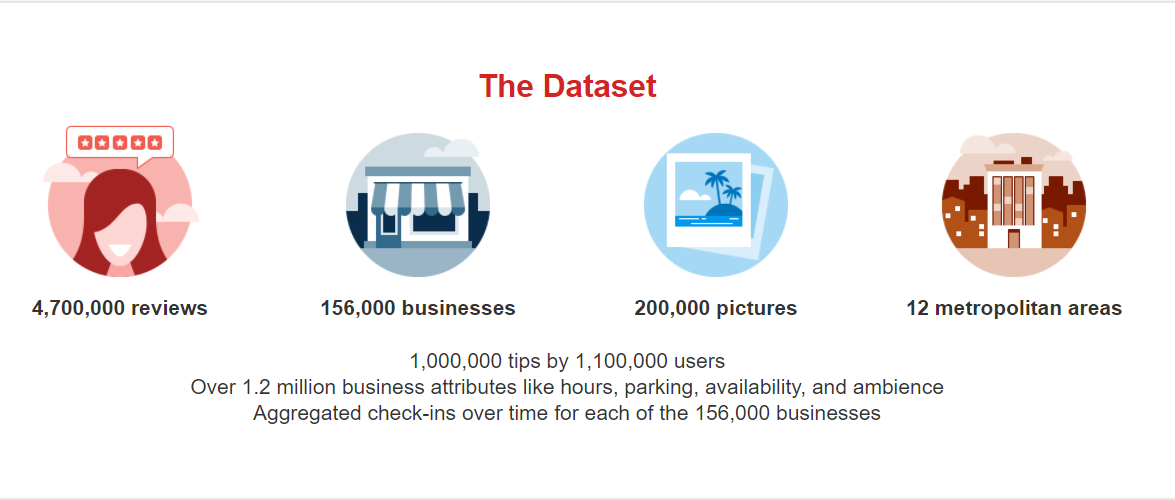
\includegraphics[scale=0.5]{data_details.png}
		\caption{Dataset Details}
	\end{figure}
	
	
	\bigskip
	
	\noindent\textbf{Methods:}
	We plan to use three different techniques for building a recommendation system and compare their performance on yelp dataset. The methods which we intend to use for building the model are Collaborative filtering\cite{cfilter}, Clustering and deep learning \cite{ydeep}.
	\bigskip
	
	\noindent\textbf{Questions:}
	Some initial questions which we plan to address. We may add more questions in future.
	\begin{itemize}
		\item Suggest a resturant based to user based on his earlier review.
		\item Find most popular business in a city in different business categories. 
		\item Find which type of cusine are more related to each other based on user rating.
	\end{itemize}
	\bigskip
	
	\noindent\textbf{Division of Work:}
	We initially want to work together on pre-processing and basis analysis of the dataset. Then each of us want to pick a technique and work on building a model using that method.
	\begin{thebibliography}{9}
		% NOTE: change the "9" above to "99" if you have MORE THAN 10 references.
		
		\bibitem{yelp} Yelp Dataset Challenge \url{https://www.yelp.com/dataset_challenge}
		\bibitem{cfilter}Collaborative filtering \url{https://en.wikipedia.org/wiki/Collaborative_filtering}
		\bibitem{ydeep} Paul Covington, Jay Adams, Emre Sargin \textit{Deep Neural Networks for YouTube Recommendations}, ACM 2016.

		
	\end{thebibliography}
	
	%%%%%%%%%%%%%%%%%%%%%%%%%%%%%%%%%%%%%%%%%
	
	
	
	
	
	
\end{document} 
